\documentclass[11pt]{article}

\usepackage[a4paper,margin=1in]{geometry}
\usepackage{amsmath,amssymb,amsthm}
\usepackage{graphicx}
\usepackage{booktabs}
\usepackage{siunitx}
\usepackage[numbers,sort&compress]{natbib}
\usepackage{xcolor}
\usepackage[colorlinks=true,allcolors=blue!55!black]{hyperref}
\usepackage{bm}
\usepackage{caption}
\captionsetup{font=small,labelfont=bf}

\newtheorem{definition}{Definition}
\newtheorem{proposition}{Proposition}

\newcommand{\R}{\mathbb{R}}
\newcommand{\bx}{\bm{x}}
\newcommand{\bxi}{\bm{\xi}}
\newcommand{\bg}{\bm{g}}
\newcommand{\bc}{\bm{c}}
\newcommand{\bff}{\bm{f}}
\newcommand{\bz}{\bm{z}}
\newcommand{\norm}[1]{\left\lVert#1\right\rVert}
\newcommand{\abs}[1]{\left\lvert#1\right\rvert}
\newcommand{\diag}{\operatorname{diag}}
\DeclareMathOperator{\vol}{vol}

\title{\bfseries Set-Based Uncertainty Propagation in Orbital Dynamics:\\
Automatic Domain Splitting over Zonotopes and Polynomial Zonotopes}

\author{}
\date{\today}

\begin{document}
\maketitle

\begin{abstract}
Propagating an initial-condition uncertainty set through nonlinear orbital
dynamics is a core problem in space situational awareness, conjunction
assessment, and orbit determination. Linear (covariance) propagation is cheap
but loses validity as nonlinearity grows; Monte Carlo is general but expensive
and noisy in the tails. Differential-algebra (DA) methods occupy the middle
ground by propagating a truncated Taylor expansion of the flow map, and
\emph{automatic domain splitting} (ADS) restores accuracy by subdividing the
domain wherever the expansion stops converging. We observe that the object ADS
manipulates---a Taylor flow map over a bounded domain of expansion
variables---is exactly a \emph{polynomial zonotope}, the set representation
developed independently in the reachability-analysis community. Building on this
correspondence, we study three usage patterns for combining ADS with zonotopic
representations on the planar two-body problem: (i)~\emph{oriented} domains, in
which the factor frame is a general parallelotope rather than an axis-aligned
box, reducing the leaf count for correlated uncertainty; (ii)~\emph{flow-aligned}
domains, in which the orientation of an ellipsoidal initial set is chosen from
the singular vectors of the state-transition matrix; and (iii)~\emph{curved}
initial sets, in which the initial geometry is itself a polynomial zonotope, as
arises when a Gaussian in orbital elements is expressed in Cartesian state. All
results are validated against $10^4$ Monte Carlo samples. The combined approach
reproduces the propagated set to the requested tolerance while using far fewer
sub-domains than an axis-aligned box, and the curved representation captures
non-Gaussian initial uncertainty that no affine set can represent.
\end{abstract}

\section{Introduction}

A recurring task in astrodynamics is to map a set of possible initial states
through the equations of motion and characterise the resulting set of possible
final states. The set may encode navigation uncertainty, manoeuvre dispersions,
an admissible region for a too-short-arc detection, or the family of states
consistent with an observation. Once the set is propagated, downstream questions
follow: does it intersect a keep-out volume, what is the collision probability,
where should a follow-up observation point.

Three families of methods dominate practice~\citep{luo2017review}. \emph{Linear
covariance} propagation maps a Gaussian through the state-transition matrix; it
is inexpensive but assumes the dynamics are well approximated by their
linearisation over the support of the distribution, which fails for large sets
or long horizons~\citep{junkins1996non}. \emph{Monte Carlo} samples the initial
distribution and propagates each sample; it is asymptotically exact and
trivially parallel but converges slowly and is noisy precisely in the
low-probability tails that matter for risk. Between the two,
\emph{differential-algebra} (DA) methods propagate a truncated Taylor expansion
of the flow map about a reference, yielding a polynomial that can be evaluated
anywhere in the domain~\citep{berz1999modern, dilizia2008application,
armellin2010asteroid, valli2013nonlinear}. The polynomial is accurate only while
the Taylor series converges over the domain; \emph{automatic domain splitting}
(ADS) recovers accuracy for large sets by subdividing the domain whenever the
truncation error of the current expansion exceeds a threshold, so that the
propagated set is described by a union of polynomial pieces, each valid on its
sub-domain~\citep{wittig2015propagation, losacco2024low}.

In parallel, the formal-verification and control communities developed
\emph{set propagation} techniques for reachability analysis, with a hierarchy of
set representations: intervals, \emph{zonotopes}~\citep{girard2005reachability},
\emph{polynomial zonotopes}~\citep{althoff2013reachability,
kochdumper2021sparse}, and their constrained
generalisations~\citep{scott2016constrained, kochdumper2023constrained}; see
\citet{althoff2021set} for a survey. The central observation of this paper is
that the DA flow map propagated by ADS \emph{is} a polynomial zonotope
(Section~\ref{sec:representations}). This identification makes the machinery of
zonotopic representations---in particular the freedom to choose the geometry of
the factor domain---available to orbital-uncertainty propagation, and conversely
gives the reachability representations an adaptive, error-driven subdivision
strategy in ADS.

We study three concrete usage patterns and their effect on cost and accuracy,
using the planar two-body problem as a controlled test bed:
\begin{enumerate}
  \item \textbf{Oriented domains} (Section~\ref{sec:oriented}): replacing the
        axis-aligned box of factors by a general parallelotope (a zonotope)
        wraps a correlated initial set more tightly and reduces the number of
        sub-domains.
  \item \textbf{Flow-aligned domains} (Section~\ref{sec:adaptive}): for an
        ellipsoidal (covariance) initial set, the covering parallelotope is free
        to orient; choosing its orientation from the singular value
        decomposition of the state-transition matrix conditions the propagated
        set and minimises subdivision.
  \item \textbf{Curved initial sets} (Section~\ref{sec:curved}): when the
        uncertainty is Gaussian in one coordinate system and expressed in
        another through a nonlinear map (e.g.\ orbital elements to Cartesian
        state), the initial set is itself a polynomial zonotope. Representing it
        as such captures non-Gaussian structure that an affine set cannot.
\end{enumerate}
Every claim is checked against $10^4$ Monte Carlo samples
(Section~\ref{sec:montecarlo}). The paper concerns the \emph{usage} of these
representations for orbital dynamics; the underlying numerics are standard DA and
ADS, and the implementation is incidental to the discussion.

\section{Background}
\label{sec:background}

\subsection{Flow map and uncertainty propagation}

Consider an autonomous ordinary differential equation
\begin{equation}
  \dot{\bx} = \bff(\bx), \qquad \bx \in \R^n,
  \label{eq:ode}
\end{equation}
with flow $\varphi_t : \R^n \to \R^n$, so that $\varphi_t(\bx_0)$ is the solution
at time $t$ from initial state $\bx_0$. Given an initial set
$\mathcal{X}_0 \subset \R^n$, the propagated set is its image under the flow,
\begin{equation}
  \mathcal{X}_t = \varphi_t(\mathcal{X}_0)
  = \{\, \varphi_t(\bx_0) : \bx_0 \in \mathcal{X}_0 \,\}.
  \label{eq:propagated}
\end{equation}
If $\mathcal{X}_0$ carries a probability density $p_0$, the propagated density is
the pushforward $p_t = (\varphi_t)_\# p_0$, supported on $\mathcal{X}_t$. The
goal of set-based propagation is a tractable, accurate representation of
$\mathcal{X}_t$ (and, where needed, of $p_t$).

\subsection{Differential algebra and the Taylor flow map}
\label{sec:da}

Parametrise the initial set by a vector of \emph{factors}
$\bxi \in [-1,1]^p$ through a map $\bx_0(\cdot) : [-1,1]^p \to \R^n$, so that
$\mathcal{X}_0 = \bx_0([-1,1]^p)$. Composing with the flow defines the
\emph{flow map}
\begin{equation}
  \mathcal{T}_t(\bxi) = \varphi_t\big(\bx_0(\bxi)\big),
  \label{eq:flowmap}
\end{equation}
whose image is exactly $\mathcal{X}_t$. Differential algebra computes the
order-$N$ Taylor expansion of $\mathcal{T}_t$ about $\bxi = \bm{0}$ by carrying
truncated polynomials through every arithmetic operation of the numerical
integrator~\citep{berz1999modern}. The result is a polynomial
\begin{equation}
  \mathcal{P}_t(\bxi) = \sum_{\abs{\bm{\alpha}} \le N}
    \bm{c}_{\bm{\alpha}}\, \bxi^{\bm{\alpha}},
  \qquad \bxi^{\bm{\alpha}} = \prod_{k=1}^{p} \xi_k^{\alpha_k},
  \label{eq:poly}
\end{equation}
with vector coefficients $\bm{c}_{\bm{\alpha}} \in \R^n$ indexed by multi-indices
$\bm{\alpha} \in \mathbb{N}_0^p$. The truncation error
$\mathcal{T}_t - \mathcal{P}_t$ is governed by the magnitude of the
highest-retained-order terms and grows as the domain deforms under the
flow~\citep{wittig2015propagation}. Evaluating~\eqref{eq:poly} at any
$\bxi \in [-1,1]^p$ predicts the propagated state of the corresponding initial
condition without re-integration; this is the property that makes a single DA
propagation stand in for many trajectories~\citep{valli2013nonlinear}.

\subsection{Test bed: the planar two-body problem}
\label{sec:twobody}

We use the planar Kepler problem in canonical units
($\mu = 1$, semi-major axis $a = 1$),
\begin{equation}
  \ddot{\bm{r}} = -\frac{\bm{r}}{\norm{\bm{r}}^3}, \qquad
  \bm{r} = (x, y),
  \label{eq:kepler}
\end{equation}
with state $\bx = (x, y, v_x, v_y)$. The reference orbit has eccentricity
$e = 0.5$ and is taken at periapsis,
$x(0) = a(1-e) = 0.5$, $v_y(0) = \sqrt{(1+e)/(1-e)} = \sqrt{3}$, with the
remaining components zero; its period is $T = 2\pi$. The two-body problem is an
informative test bed because its nonlinearity is strong near periapsis and mild
near apoapsis, so the difficulty of propagation varies along a single orbit, and
because exact references are available for validation. All DA propagations below
use truncation order $N = 8$ and an adaptive Runge--Kutta integrator with
tolerance $10^{-12}$.

\section{Set representations}
\label{sec:representations}

We summarise the relevant representations, each describing a set as the image of
the factor box $[-1,1]^p$ under a map of increasing generality, and make precise
the identification used throughout.

\begin{definition}[Interval / box]
A box is the image of the factor cube under a diagonal affine map,
\begin{equation}
  \mathcal{B} = \{\, \bc + \diag(\bm{h})\,\bxi : \bxi \in [-1,1]^p \,\},
  \label{eq:box}
\end{equation}
with centre $\bc$ and half-widths $\bm{h}$. It can stretch only along the
coordinate axes.
\end{definition}

\begin{definition}[Zonotope~\citep{girard2005reachability}]
A zonotope replaces the diagonal by a general \emph{generator matrix}
$G \in \R^{n\times p}$,
\begin{equation}
  \mathcal{Z} = \{\, \bc + G\,\bxi : \bxi \in [-1,1]^p \,\}
  = \bc \oplus \bigoplus_{j=1}^{p} [-1,1]\, \bg_j,
  \label{eq:zono}
\end{equation}
i.e.\ the Minkowski sum of the line segments spanned by the generator columns
$\bg_j$. When $p = n$ and $G$ is nonsingular, $\mathcal{Z}$ is a
\emph{parallelotope}: an affine image of the cube, free to rotate and shear. A
box is the special case $G = \diag(\bm{h})$. Every zonotope is convex and
centrally symmetric about $\bc$.
\end{definition}

\begin{definition}[Polynomial zonotope~\citep{althoff2013reachability,
kochdumper2021sparse}]
A polynomial zonotope lets the factors enter through a polynomial,
\begin{equation}
  \mathcal{PZ} = \Big\{\, \bc + \sum_{i=1}^{h}
    \Big(\textstyle\prod_{k=1}^{p} \xi_k^{E_{ki}}\Big)\, \bg_i
    : \bxi \in [-1,1]^p \,\Big\},
  \label{eq:pz}
\end{equation}
with an exponent matrix $E \in \mathbb{N}_0^{p \times h}$ and generators
$\bg_i \in \R^n$. Unlike a zonotope, a polynomial zonotope can be non-convex and
asymmetric; it can bend and fold.
\end{definition}

Comparing~\eqref{eq:poly} and~\eqref{eq:pz} gives the identification that
organises this paper.

\begin{proposition}
\label{prop:identification}
The truncated DA flow map $\mathcal{P}_t$ of~\eqref{eq:poly}, regarded as a set
over $\bxi \in [-1,1]^p$, is a polynomial zonotope: its centre is the constant
term $\bm{c}_{\bm 0}$, its generators are the nonconstant coefficients
$\bm{c}_{\bm{\alpha}}$, and its exponent matrix collects the corresponding
multi-indices $\bm{\alpha}$.
\end{proposition}

Thus DA propagation produces a polynomial zonotope per domain, and the
single-segment objects~\eqref{eq:box}--\eqref{eq:zono} are the degree-one special
cases used to describe the \emph{initial} set or to over-approximate the
propagated one. Constrained zonotopes~\citep{scott2016constrained} and
constrained polynomial zonotopes~\citep{kochdumper2023constrained} extend the
hierarchy with equality constraints $A\bxi = \bm{b}$ on the factors, which can
represent arbitrary convex polytopes and lower-dimensional sub-manifolds; they
are not used in the experiments below but are relevant to the applications
discussed in Section~\ref{sec:discussion}.

Figure~\ref{fig:representations} illustrates the hierarchy on an explicit
degree-two map
$\bm\varphi(p,q) = (\,p + \tfrac12 q + 0.35\,q^2,\; q + 0.45\,p^2 - 0.25\,pq\,)$
applied to a square of initial conditions. Because the map is degree two and
$N \ge 2$, the polynomial zonotope coincides with the true image (the Monte
Carlo cloud fills it exactly); the box is a loose enclosure, and the linear
(zonotope) image---an affine map of the box---cannot reproduce the curvature. The
right panels show that subdividing the factor box and taking the per-piece linear
image converges onto the curved set: this is the geometric content of automatic
domain splitting.

\begin{figure}[t]
  \centering
  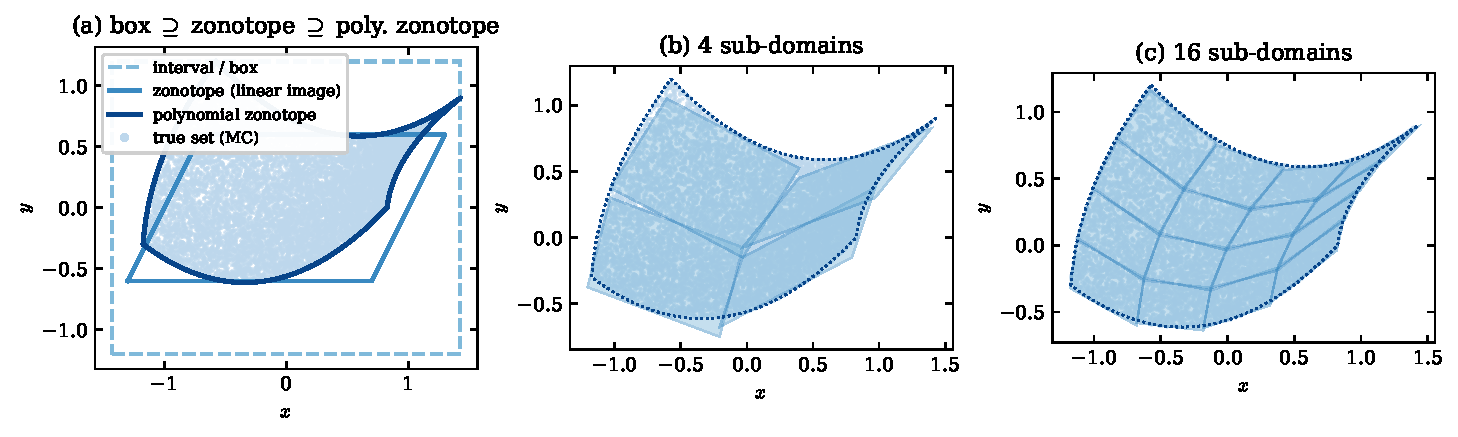
\includegraphics[width=\textwidth]{figures/fig_representations.pdf}
  \caption{Set representations on a degree-two map. (a)~The polynomial zonotope
  (darkest) coincides with the true set (pale points); the box (dashed) is a
  loose enclosure and the linear zonotope image misses the curvature.
  (b,c)~Subdividing the factor box and taking each piece's linear image
  converges onto the curved set---the principle behind ADS. All shades are drawn
  from the \textsf{Blues} colormap.}
  \label{fig:representations}
\end{figure}

\section{Automatic domain splitting}
\label{sec:ads}

ADS makes the polynomial representation reliable for large sets by subdividing
the factor domain~\citep{wittig2015propagation}. Let
$m_N(\mathcal{P}) = \sum_{\abs{\bm{\alpha}} = N} \norm{\bm{c}_{\bm{\alpha}}}_1$
denote the total magnitude of the highest-order coefficients, a proxy for the
truncation error over $[-1,1]^p$. The driver integrates the flow map and, at
each accepted step, tests $m_N$ against a tolerance $\varepsilon$. If
$m_N > \varepsilon$ the domain is bisected along the factor $\xi_d$ that
contributes most of $m_N$; otherwise the leaf is accepted.

Bisection along $\xi_d$ replaces the factor by two half-ranges through the affine
substitution
\begin{equation}
  \xi_d \;\mapsto\; \pm\tfrac12 + \tfrac12\,\xi_d',
  \label{eq:split}
\end{equation}
applied to the polynomial~\eqref{eq:poly}; expanding
$(\pm\tfrac12 + \tfrac12 \xi_d')^{\alpha_d}$ by the binomial theorem
re-expresses the flow map in the child's local coordinates without
re-integration. Each child is again a polynomial zonotope on its sub-box, and
the process recurses until every leaf satisfies the tolerance or a maximum depth
is reached. The output is a tree whose leaves tile the propagated set: a
\emph{piecewise polynomial zonotope}. The low-order variant LOADS replaces the
truncation-mass criterion by a nonlinearity index built from the variation of
the Jacobian, which can reduce the expansion order needed for a given
accuracy~\citep{losacco2024low}.

Figure~\ref{fig:ads} shows ADS applied to a box of initial conditions on the
two-body orbit, with leaves shaded by their subdivision depth. The partition is
coarse where the flow is mild and fine where periapsis passage stretches the
set; the leaf count grows accordingly along the orbit.

\begin{figure}[t]
  \centering
  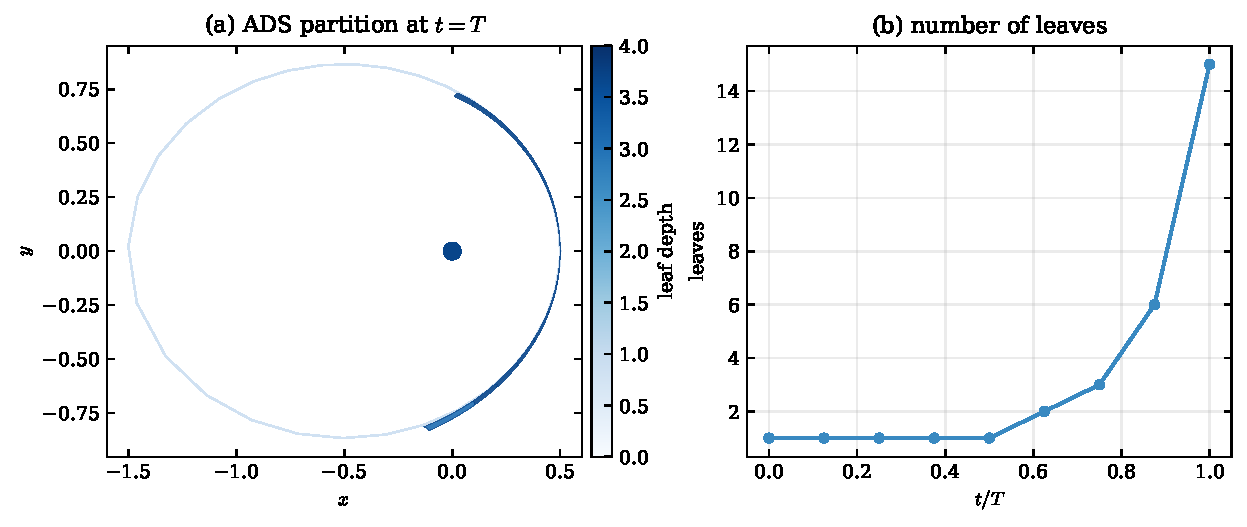
\includegraphics[width=0.86\textwidth]{figures/fig_ads_partition.pdf}
  \caption{Automatic domain splitting on a two-body initial-condition box.
  (a)~Leaves of the partition at $t = T$, shaded by subdivision depth; the
  partition refines where the dynamics are most nonlinear. (b)~Number of leaves
  along the orbit.}
  \label{fig:ads}
\end{figure}

\section{Oriented domains}
\label{sec:oriented}

The DA flow map and the substitution~\eqref{eq:split} operate entirely in the
normalised factors $\bxi$; they are unaffected by how those factors map to
physical initial states. That mapping---the geometry of the initial
set---therefore can be chosen freely. The classical choice is the axis-aligned
box~\eqref{eq:box}. Replacing it by a parallelotope~\eqref{eq:zono} with a
general generator matrix $G$ lets a single domain wrap a \emph{correlated} or
rotated initial set that a box would have to over-bound. Because subdivision
bisects a generator (a column of $G$), the cuts follow the oriented directions of
the set rather than the coordinate axes.

The effect is a smaller leaf count. Consider a two-body uncertainty in
$(y, v_y)$ shaped as a parallelogram rotated by $45^\circ$, and compare its
propagation as an oriented zonotope against the axis-aligned box that bounds the
same set. Over a representative arc the oriented domain needs fewer leaves at
every snapshot (e.g.\ $48$ versus $75$ near mid-arc), because the bounding box
covers empty corners that carry additional truncation mass and trigger spurious
splits (Figure~\ref{fig:oriented}). The advantage is configuration dependent: a
\emph{fixed} orientation is a gamble, and over a full period the same
$45^\circ$ frame can become misaligned with the periapsis-return shear and lose
to the box. This motivates choosing the orientation from the dynamics.

\begin{figure}[t]
  \centering
  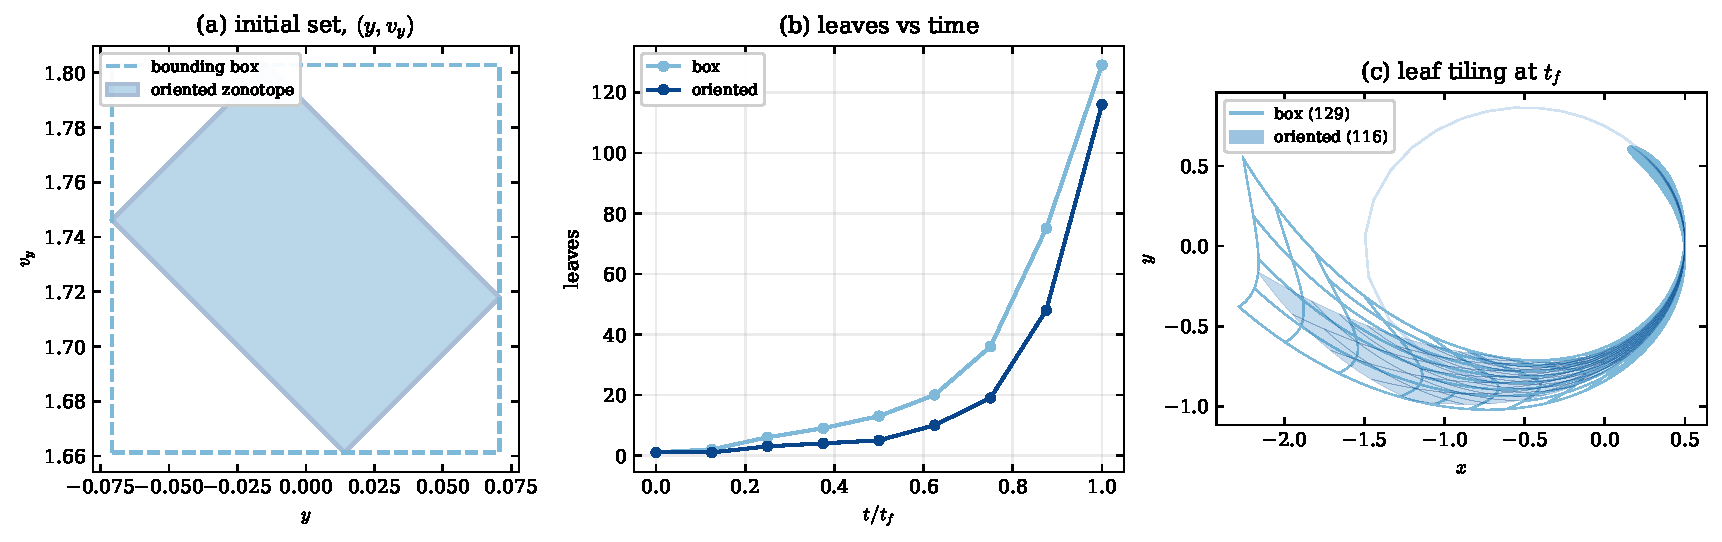
\includegraphics[width=\textwidth]{figures/fig_oriented.pdf}
  \caption{Oriented (parallelotope) versus axis-aligned (box) initial set on the
  two-body problem. (a)~The correlated initial set and its bounding box in
  $(y, v_y)$. (b)~Leaf count along the arc. (c)~Leaf tiling at the final time;
  the box wastes leaves on the region its bound includes, while the oriented
  domain hugs the propagated set.}
  \label{fig:oriented}
\end{figure}

\section{Flow-aligned domains}
\label{sec:adaptive}

When the initial uncertainty is an \emph{ellipsoid}---a covariance
$\Sigma = LL^\top$---the covering parallelotope is free to orient, because an
ellipsoid has no preferred generator frame: for any orthogonal $V$, the
parallelotope $\{\bc + LV\bxi : \bxi \in [-1,1]^p\}$ contains the same ellipsoid
(the unit ball is contained in the unit cube, and $V$ maps the cube to a set
still containing the ball). This freedom can be spent to condition the
\emph{propagated} set.

Let $\Phi = \partial \varphi_T / \partial \bx_0$ be the state-transition matrix
(the linear part of the flow map) over the horizon, obtained from a single
un-split DA propagation. Take the thin singular value decomposition
$\Phi L = U \Sigma_s V^\top$ and choose generators $G = LV$. Then the propagated
parallelotope has linear image $\Phi G = U \Sigma_s$, whose columns are
orthogonal and ordered by stretch: the set is mapped to a well-conditioned,
axis-aligned (in the singular frame) parallelotope rather than a thin diagonal
sliver that axis-aligned cuts would over-subdivide.

Figure~\ref{fig:adaptive} compares three coverings of the \emph{same} ellipsoid
over a full period: the axis-aligned bounding box, a fixed Cholesky
parallelotope (oriented by the covariance only), and the flow-aligned
parallelotope. The flow-aligned frame needs the fewest leaves at every snapshot
(\textbf{50} versus \textbf{56} for the box and \textbf{210} for the
Cholesky frame at $t = T$), \emph{fixing} the periapsis-return penalty that a
fixed orientation suffers. Notably the flow-aligned covering is \emph{larger} in
area than the box yet subdivides less: the gain is from orientation, not size,
and a poorly oriented frame (the fixed Cholesky one) is several times worse.
Re-expressing the propagated map in the aligned frame---a linear change of
factor variables applied to the polynomial---confirms that the deformation is
diagonalised: the off-diagonal of $\Phi^\top \Phi$ in the aligned frame drops
from $\approx 1.2$ to $\approx 0$.

\begin{figure}[t]
  \centering
  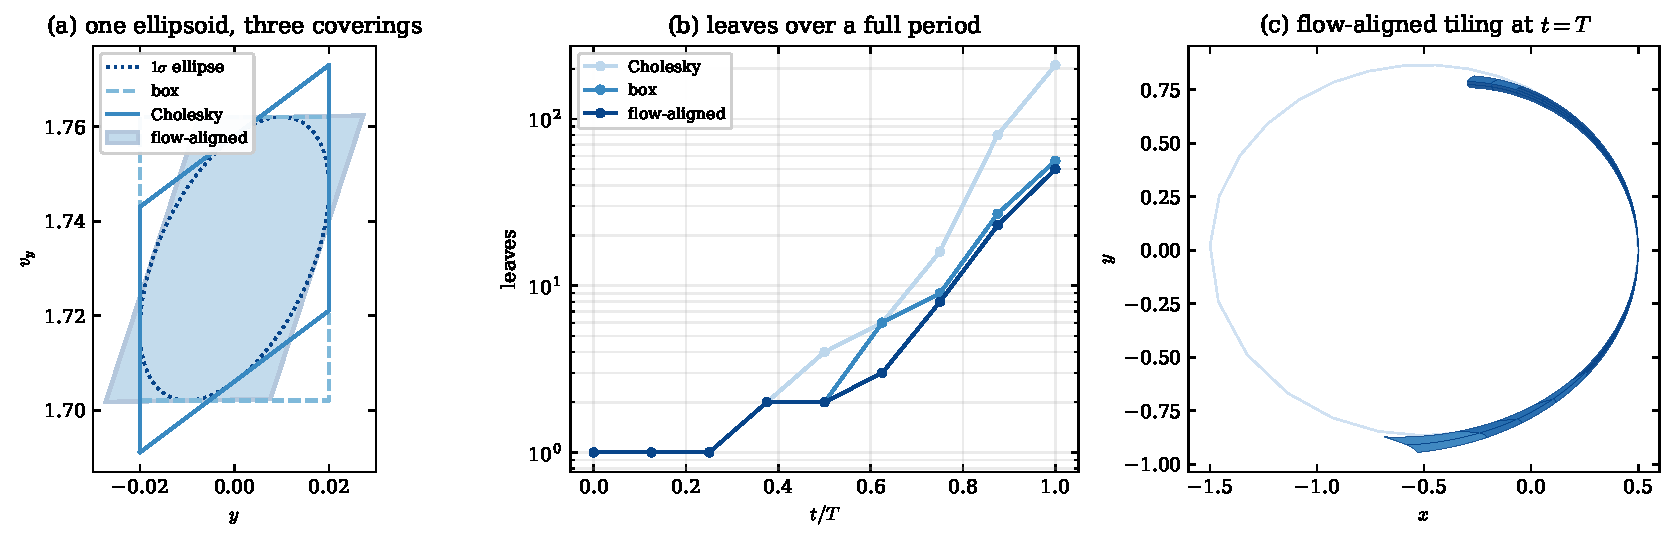
\includegraphics[width=\textwidth]{figures/fig_adaptive.pdf}
  \caption{Flow-aligned covering of a covariance ellipsoid. (a)~The
  $1\sigma$ ellipse and three parallelotope/box coverings in $(y, v_y)$.
  (b)~Leaf count over a full period (log scale): the flow-aligned frame is
  lowest throughout, the misaligned Cholesky frame highest. (c)~The flow-aligned
  partition at $t = T$, shaded by depth.}
  \label{fig:adaptive}
\end{figure}

A geometric caveat bounds how far the orientation can be pushed. A linear change
of factor variables $\bxi = R\bm{\eta}$ maps the cube $[-1,1]^p$ to
$R[-1,1]^p$, which is a cube again only when $R$ is a signed permutation.
Re-orienting the frame of a \emph{fixed} parallelotope therefore either changes
the represented set or requires an over-approximation back to a cube. The
construction above is exact precisely because an ellipsoid leaves the covering
parallelotope free to orient; for a covariance the orientation is chosen once,
up front, from the horizon $\Phi$.

\section{Curved initial sets}
\label{sec:curved}

The representations so far take an affine \emph{initial} geometry and let the
flow introduce curvature. But the initial uncertainty itself is often curved.
This is the generic situation when the uncertainty is Gaussian in one coordinate
system and required in another: an admissible region in range/range-rate, a
Gaussian in orbital elements expressed in Cartesian state, or a phase
uncertainty along an orbit. We ask what a linear initial representation can and
cannot do, and use a polynomial-zonotope initial set instead.

\paragraph{Why an affine set cannot represent a curved one.}
A linear initial set is $\bx_0(\bxi) = \bc + G\bxi$, an affine image of the box,
hence a parallelotope: flat faces, straight edges, central symmetry about $\bc$.
That is the entire expressive range of a linear or covariance representation. Let
the true initial map be $\bm{g} : [-1,1]^p \to \R^n$, and expand it about the
centre,
\begin{equation}
  \bx_0(\bxi) = \bm{g}(\bm 0) + J\bxi
    + \tfrac12\,\big(\bxi^\top H_i \bxi\big)_{i=1}^{n} + \cdots,
  \label{eq:curved-expand}
\end{equation}
with Jacobian $J$ and component Hessians $H_i$. The best linear representation
keeps only $\bc + J\bxi$ and lies on the tangent plane at the centre; the true
set departs from it by the quadratic term. Scaling the factors so that
$\bxi = \pm\bm{1}$ corresponds to the $3\sigma$ boundary, the displacement is
$\bxi \sim O(1)$, so the dropped curvature $\tfrac12 \bxi^\top H_i \bxi$ is the
\emph{same order} as the linear spread $J\bxi$ itself---not a small correction.
No affine map produces a curved, asymmetric set; the deficiency is structural,
not a matter of fitting $G$ better. A polynomial zonotope retains the
higher-order terms of~\eqref{eq:curved-expand} and bends to follow the manifold.

\paragraph{Construction.}
For the two-body problem, take the uncertainty to be a $3\sigma$ Gaussian in
true anomaly $\nu$ and eccentricity $e$ about $(\nu_0, e_0) = (0, 0.5)$, mapped
to Cartesian state through the perifocal relations
\begin{equation}
  r = \frac{a(1-e^2)}{1 + e\cos\nu}, \quad
  \bm{r} = r(\cos\nu, \sin\nu), \quad
  \dot{\bm{r}} = \sqrt{\tfrac{\mu}{a(1-e^2)}}\,(-\sin\nu,\; e + \cos\nu).
  \label{eq:perifocal}
\end{equation}
Substituting $\nu = 3\sigma_\nu\,\xi_1$ and $e = e_0 + 3\sigma_e\,\xi_2$ and
expanding~\eqref{eq:perifocal} as a DA polynomial yields a curved
polynomial-zonotope initial set $\bx_0(\bxi)$, which is propagated by ADS exactly
as before. The first-order truncation of $\bx_0$ provides the linear (tangent)
comparison, the parallelotope a covariance would supply.

\paragraph{Result.}
With $\sigma_\nu = 0.12$ (so the $3\sigma$ span is $\pm21^\circ$) and
$\sigma_e = 0.04$ ($e \in [0.38, 0.62]$), propagated to $0.75\,T$, the curved
polynomial-zonotope set is represented by \textbf{18} leaves and reproduces the
$10^4$-sample cloud with root-mean-square position error
$2.6\times10^{-3}$ (maximum $1.2\times10^{-2}$). The linear initial set, by
contrast, requires \textbf{172} leaves and attains only RMS $0.48$ (maximum
$11$): its flat $3\sigma$ geometry is wrong from the outset, and the nonlinear
flow amplifies the error---indeed its tangent set reaches near-collision states
that diverge if the horizon or the spread is pushed further. At $3\sigma$ the
curvature is not a correction but the difference between a correct answer and a
useless one (Figure~\ref{fig:curved}).

\begin{figure}[t]
  \centering
  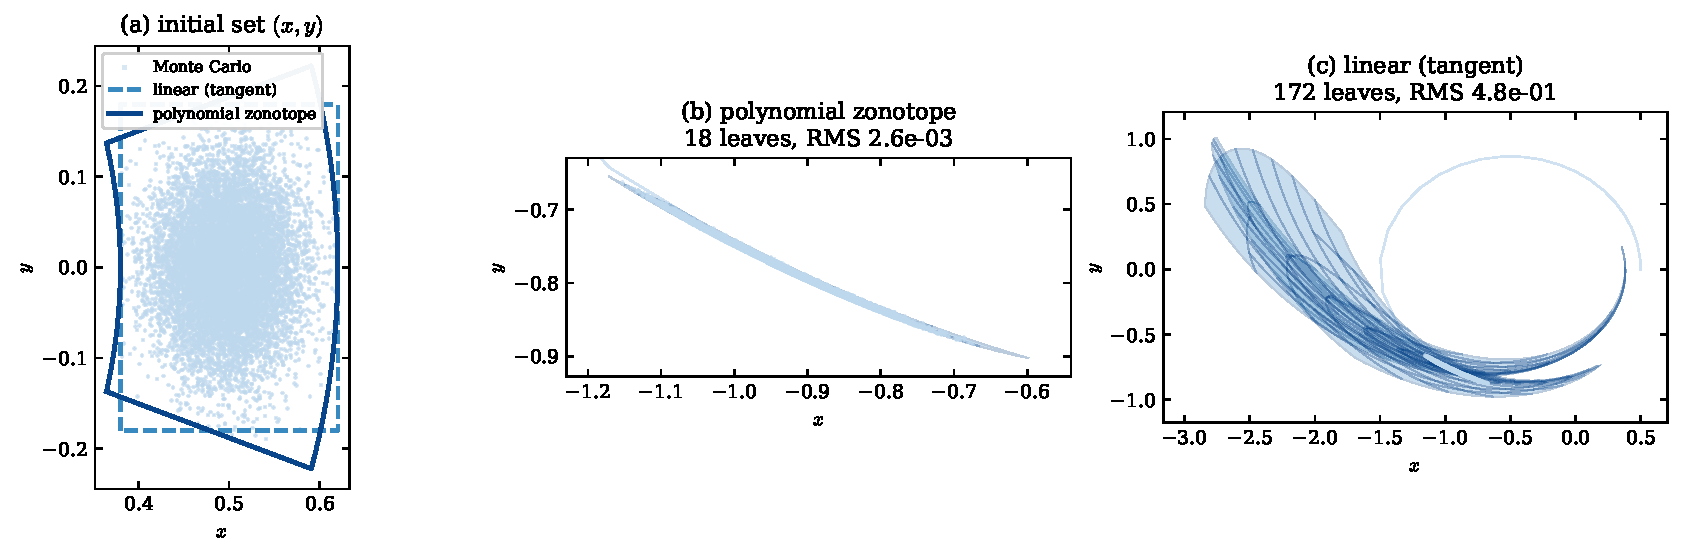
\includegraphics[width=\textwidth]{figures/fig_curved.pdf}
  \caption{Curved initial set (Gaussian in orbital elements) versus its linear
  approximation. (a)~Initial sets in $(x, y)$ over the Monte Carlo cloud: the
  polynomial zonotope (solid) bends with the cloud, the tangent parallelotope
  (dashed) is flat. (b)~Propagated, the curved set tracks the cloud with
  $18$ leaves. (c)~The linear set, propagated, smears far past the cloud
  ($172$ leaves).}
  \label{fig:curved}
\end{figure}

\section{Monte Carlo validation}
\label{sec:montecarlo}

To confirm that the piecewise polynomial zonotope does not merely \emph{bound}
the propagated set but \emph{reproduces} it, we draw $10^4$ samples from each
initial distribution, propagate them with a high-accuracy integrator, locate the
leaf containing each sample, evaluate that leaf's flow map, and measure the
prediction error. Figure~\ref{fig:mc} overlays the partition on the cloud for the
ellipsoidal case; the leaf tilings envelope the samples in every covering.

Table~\ref{tab:mc} collects leaf counts and errors. All coverings reproduce the
cloud to the split tolerance, so the choice of domain geometry is a question of
\emph{cost} (leaf count) rather than achievable accuracy---except for the linear
\emph{initial} set, which cannot represent the curved geometry and is therefore
inaccurate at any leaf count. The flow-aligned covering attains both the fewest
leaves and the lowest error for the ellipsoidal case.

\begin{figure}[t]
  \centering
  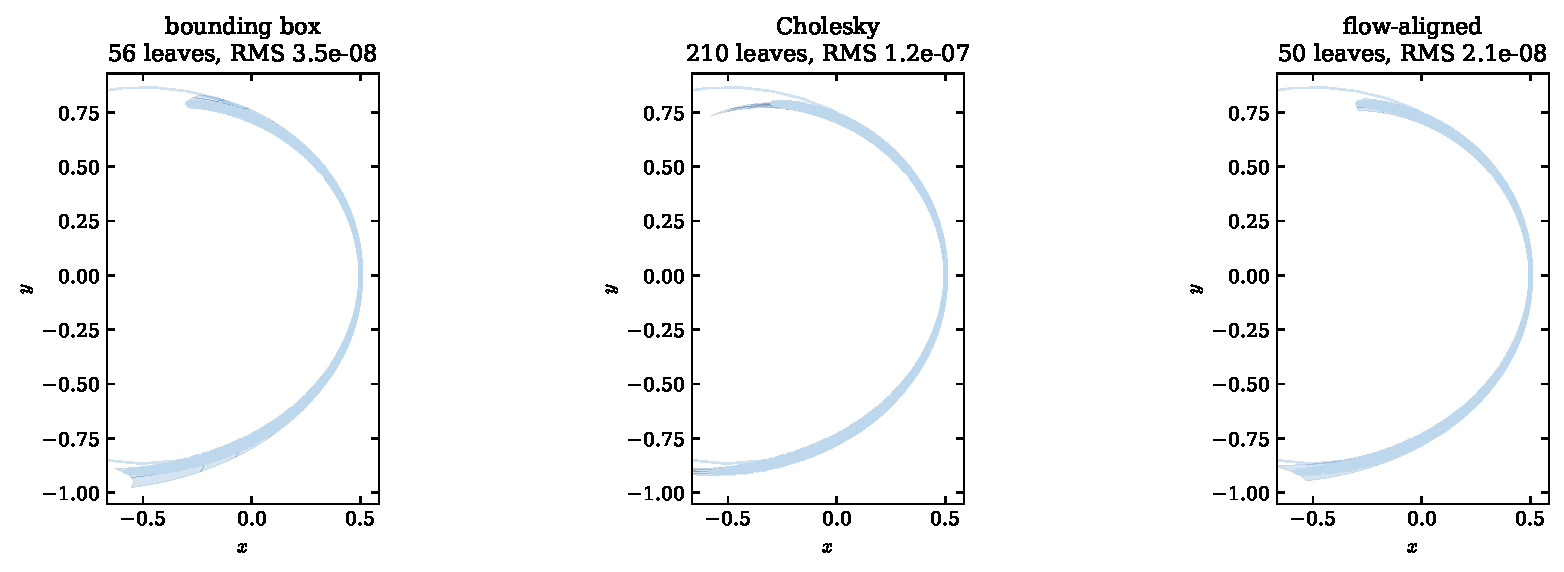
\includegraphics[width=\textwidth]{figures/fig_mc.pdf}
  \caption{Monte Carlo validation for the covariance-ellipsoid case at $t = T$:
  the leaf tiling of each covering over the $10^4$-sample cloud (pale points).
  All three envelope the cloud; the leaf counts differ.}
  \label{fig:mc}
\end{figure}

\begin{table}[t]
  \centering
  \caption{Leaf count and Monte Carlo prediction error ($10^4$ samples) for the
  domain geometries studied. Errors are position RMS / maximum over the samples.
  ``Parallelotope'' and ``ellipsoid'' refer to the initial set; ``curved'' is
  the polynomial-zonotope initial set of Section~\ref{sec:curved}.}
  \label{tab:mc}
  \small
  \begin{tabular}{llrll}
    \toprule
    Initial set & Domain geometry & Leaves & RMS error & Max error \\
    \midrule
    Parallelotope ($0.8\,T$) & bounding box        & 129 & \num{4.7e-8} & \num{5.2e-7} \\
                             & oriented zonotope   & \textbf{116} & \num{1.1e-7} & \num{1.9e-6} \\
    \addlinespace
    Ellipsoid ($T$)          & bounding box        & 56  & \num{3.5e-8} & \num{3.8e-7} \\
                             & Cholesky frame      & 210 & \num{1.2e-7} & \num{3.4e-6} \\
                             & flow-aligned        & \textbf{50}  & \num{2.1e-8} & \num{2.5e-7} \\
    \addlinespace
    Curved ($0.75\,T$)       & polynomial zonotope & \textbf{18}  & \num{2.6e-3} & \num{1.2e-2} \\
                             & linear (tangent)    & 172 & \num{4.8e-1} & \num{1.1e1} \\
    \bottomrule
  \end{tabular}
\end{table}

\section{Discussion}
\label{sec:discussion}

\paragraph{Choosing a representation.}
The experiments suggest a simple decision rule. For a \emph{filled, affine}
uncertainty (a box or a covariance ellipsoid), the propagated set is recovered by
ADS over a box; an \emph{oriented} parallelotope reduces the leaf count when the
set is correlated or anisotropic, and for an ellipsoid the orientation is best
taken from the state-transition matrix, which is exact and cheap. For a
\emph{curved} initial uncertainty---non-Gaussian in the working coordinates---a
polynomial-zonotope initial set is required: no affine geometry can represent it,
and using one produces both more leaves and a wrong answer.

\paragraph{On the $3\sigma$ ellipse.}
A filled $3\sigma$ ellipse is full-dimensional and needs no constraints; the
oriented/flow-aligned covering of Section~\ref{sec:adaptive} handles it.
Constraints~\citep{scott2016constrained, kochdumper2023constrained} become useful
when the question concerns a \emph{sub-manifold} of the ellipse rather than the
whole set: its $3\sigma$ \emph{shell} (a single quadratic constraint, the
worst-case contour); a stiff direction of a rank-deficient covariance; or the
sub-population that triggers an event at a later time, i.e.\ the preimage
$\{\bxi : \varphi_T(\bx_0(\bxi)) \in \mathcal{G}\}$ of a keep-out or
close-approach region $\mathcal{G}$, which pulls back through the leaf polynomial
to a polynomial constraint on the factors. Because the constraint lowers the
dimension, it both reduces the number of sub-domains and sharpens the answer; the
collision probability is then an integral of the initial Gaussian over the
constrained factor region rather than a Monte Carlo hit count. These are natural
extensions of the present work.

\paragraph{Cost and limitations.}
The cost of a curved (polynomial-zonotope) domain is that each leaf carries its
initial map in addition to the propagated one, roughly doubling per-leaf memory,
and exact point location requires inverting a polynomial map (we use a
first-order inverse on the small leaves). The flow-aligned construction assumes
an ellipsoidal initial set and a single horizon-level orientation; time-varying
re-orientation would require an over-approximation, as noted in
Section~\ref{sec:adaptive}. Finally, the present study is two-dimensional in the
uncertain factors and uses a single dynamical model; the representations carry
over to higher factor dimension and to perturbed dynamics without change, but the
leaf-count scaling with factor dimension---the curse that ADS shares with all
grid-like subdivisions---remains the practical limit.

\section{Conclusion}

We identified the DA flow map propagated by automatic domain splitting with the
polynomial zonotope of reachability analysis, and used that identification to
study three usage patterns on the two-body problem: oriented domains for
correlated sets, flow-aligned domains for covariance ellipsoids, and curved
polynomial-zonotope initial sets for non-Gaussian uncertainty. Validated against
$10^4$ Monte Carlo samples, the combined approach reproduces the propagated set
to tolerance while using markedly fewer sub-domains than an axis-aligned box, and
the curved representation captures initial uncertainty that no affine set can.
The set-representation hierarchy developed for formal verification and the
adaptive, error-driven subdivision developed for astrodynamics are complementary,
and their combination is a practical tool for nonlinear orbital-uncertainty
propagation.

\bibliographystyle{plainnat}
\bibliography{references}

\end{document}
